%; whizzy chapter
% -initex iniptex -latex platex -format platex -bibtex jbibtex -fmt fmt
% 以上 whizzytex を使用する場合の設定。

%     Kansai Debian Meeting resources
%     Copyright (C) 2007 Takaya Yamashita
%     Thank you for Tokyo Debian Meeting resources

%     This program is free software; you can redistribute it and/or modify
%     it under the terms of the GNU General Public License as published by
%     the Free Software Foundation; either version 2 of the License, or
%     (at your option) any later version.

%     This program is distributed in the hope that it will be useful,
%     but WITHOUT ANY WARRANTY; without even the implied warranty of
%     MERCHANTABILITY or FITNESS FOR A PARTICULAR PURPOSE.  See the
%     GNU General Public License for more details.

%     You should have received a copy of the GNU General Public License
%     along with this program; if not, write to the Free Software
%     Foundation, Inc., 51 Franklin St, Fifth Floor, Boston, MA  02110-1301 USA

%  preview (shell-command (concat "evince " (replace-regexp-in-string "tex$" "pdf"(buffer-file-name)) "&"))
% 画像ファイルを処理するためにはebbを利用してboundingboxを作成。
%(shell-command "cd image200708; ebb *.png")

%%ここからヘッダ開始。

\documentclass[mingoth,a4paper]{jsarticle}
\usepackage{kansaimonthlyreport}
\usepackage[dvips]{xy}
\usepackage{ulem}
\usepackage{eurosym}

% 日付を定義する、毎月変わります。
\newcommand{\debmtgyear}{2013}
\newcommand{\debmtgdate}{27}
\newcommand{\debmtgmonth}{1}
\newcommand{\debmtgnumber}{68}

\begin{document}

\begin{titlepage}

% 毎月変更する部分、本文の末尾も修正することをわすれずに

 第\debmtgnumber{}回 関西 Debian 勉強会資料

\vspace{2cm}

\begin{center}
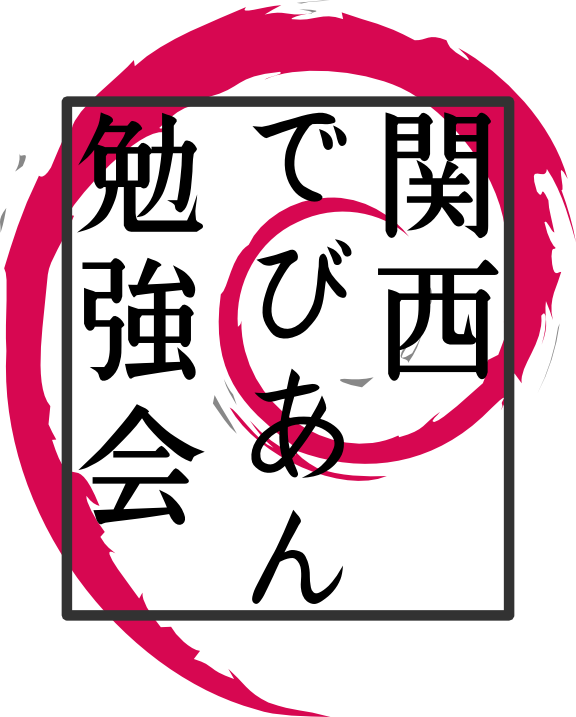
\includegraphics{image200802/kansaidebianlogo.png}
\end{center}

\begin{flushright}
\hfill{}関西 Debian 勉強会担当者 佐々木・倉敷・のがた・かわだ \\
\hfill{}\debmtgyear{}年\debmtgmonth{}月\debmtgdate{}日
\end{flushright}

\thispagestyle{empty}
\end{titlepage}

\dancersection{Introduction}{Debian JP}

\vspace{1em}

 関西Debian勉強会はDebian GNU/Linuxのさまざまなトピック
 (新しいパッケージ、Debian特有の機能の仕組、Debian界隈で起こった出来事、
 などなど)について話し合う会です。

 目的として次の三つを考えています。
 \begin{itemize}
  \item MLや掲示板ではなく、直接顔を合わせる事での情報交換の促進
  \item 定期的に集まれる場所
  \item 資料の作成
 \end{itemize}

 それでは、楽しい一時をお楽しみ下さい。

\newpage

\begin{minipage}[b]{0.2\hsize}
 {\rotatebox{90}{\fontsize{80}{80}
{\gt 関西 Debian 勉強会}}}
\end{minipage}
\begin{minipage}[b]{0.8\hsize}
\hrule
\vspace{2mm}
\hrule
\setcounter{tocdepth}{1}
\tableofcontents
\vspace{2mm}
\hrule
\end{minipage}

\dancersection{最近のDebian関係のイベント報告}{Debian JP}

\subsection{第 67 回関西 Debian 勉強会}

67 回目の関西 Debian 勉強会は 12 月 23 日に福島区民センターで行ないました。

「Android 端末(Asus Transformer TF201)への Debian インストール奮闘記」と
「月刊 Debian Policy パッケージ管理スクリプトとインストール手順」、「2012年の振り返りと2013年の企画」といった内容でした。

Android で実用できる Debian 環境が構築されていましたが、その後も気になるところです。unstable 環境にアップグレードできたのでしょうか。

月刊 Debian Policy は一年でようやく半分終わって、残りは重たい内容ばかりになってきました。
残り今年も続けていきましょう。Policy 読んでみたい方お待ちしております。

2013年の企画もお待ちしていますよ。


\subsection{第 96 回東京エリア Debian 勉強会}
96 回目の東京エリア Debian 勉強会は 1 月 16 日にスクウェア・エニックスで開催されました。

「Debian予約システムアンケート集計」、「gdbのpython拡張(その1)」「月刊Debhelper」といった内容でした。

Debian 予約システムのアンケート機能のフィードバックから、未回答のアンケートへのリンクが登録一覧のところに表示されるようになりましたので確認してみてください。

予約システムへの要望があれば言ってみると反映されていくかもしれませんよ。


\subsection{福岡 Debian 勉強会 2 回目}
2 回目の福岡 Debian 勉強会が 1 月 26 日に開催されました。
「Debianに片足も両足も突っ込んだ皆さん、こんにちは(仮)」、「d-i usbメモリの作り方 or wheezyについて何か(仮)」といった内容でした。

福岡での Debian 勉強会も根付いてきたようです。各地で Debian 勉強会が開催されていくといいですね.


\dancersection{事前課題}{Debian JP}

今回は以下の課題を出題しました.
\begin{screen}
  \begin{enumerate}
  \item 2015年ではDebianはどうなっているかを大胆に予想してください。
  \item これまでDebianでどんなCMSやWebアプリフレームワークを使ったことがありますか?
  \item 本来、Debianではパッケージが提供されているならば、それを使うのが望ましいですが、あえてDebianのパッケージを使わなかった事はありますか?
  \item Drupalの標準ファイル配置は /var/www以下のドキュメントルートにすべてのファイルを一括配置します。
    http://drupalcode.org/project/drupal.git/tree/2c99f0b21755c34cffd4fc5b38161d64bd69ca8a
    Debianパッケージの場合はどう変化するか説明してください。
    どのコマンドを使えば調べられるでしょうか。
  \item 可能であれば以下のVMを動かしてみてください。(Drupalコアと重要モジュールが入った状態になっています)
    Drupal 7 - Content Management Framework
  \end{enumerate}
\end{screen}

参加者の皆さんの解答は以下の通りです。

\begin{prework}{ かわだてつたろう }
  \begin{enumerate}
  \item  -devel は相変わらず init.d の話題で炎上しているが、Jessie が滞りなくリリースされる。

    DebConf15 が日本で開催されようとしている。といいなぁ。
  \item Trac, WordPress と Symfony, CakePHP
  \item Symfony, CakePHP などのWeb アプリフレームワークはプロジェクトのソース管理に含めて管理したいので使わないことが多い。

    デプロイ環境が Debian で無かったり、root 権限が無い場合に都合がよい。
  \item debian 以下をみると次のように変更される。
    \begin{commandline}
debian/dirs
  sites			etc/drupal/7/sites/default

debian/docs
  MAINTAINERS.txt	usr/share/doc/drupal7/
  UPGRADE.txt		usr/share/doc/drupal7/
  INSTALL.mysql.txt	usr/share/doc/drupal7/
  INSTALL.pgsql.txt	usr/share/doc/drupal7/
  INSTALL.sqlite.txt	usr/share/doc/drupal7/
  README.txt		usr/share/doc/drupal7/
  scripts		usr/share/doc/drupal7/

debian/drupal7.install
  *.php			usr/share/drupal7/
  includes		usr/share/drupal7/
  misc			usr/share/drupal7/
  modules		usr/share/drupal7/
  themes		usr/share/drupal7/
  robots.txt		usr/share/drupal7/
  profiles		usr/share/drupal7/

debian/examples
  sites/default/default.settings.php	usr/share/doc/drupal7/examples/

debian/rules
  .htaccess		etc/drupal/7/htaccess

debhelper によって
  CHANGELOG.txt		usr/share/doc/drupal7/
    \end{commandline}
\item 試してみます。
  \end{enumerate}
\end{prework}

\begin{prework}{ のがたじゅん }
  \begin{enumerate}
  \item Debianなスマートフォンが出て幸せになる(とよいなぁ)
  \item パッケージで使ったのはWordpress, DokuWiki, tDiaryあたりとか。CMS/フレームワークではないけどRedmineをパッケージで入れたら、めちゃ簡単でよかったですね。
  \item 管理で楽をしたいので、なるべくならパッケージを利用したいです。パッケージを使わないときは、最新のものを使いたい時とか?
  \item apt-file searchとやってもいいけど、packages.debian.orgで検索してファイル一覧を見てみました。\footnote{\url{http://packages.debian.org/wheezy/all/drupal7/filelist}}

    {\tt /usr/share/drupal7}以下に本体があります。apacheのaliasで使うようになってますね。README.Debianを見ればセットアップ方法もわかるけど、Wordpressのパッケージに比べるとちょっと不親切かな。

    drushがパッケージになってたので、{\tt /usr/share/drupal7}以下で使ってパッケージのファイルを破壊しました(・ω<) てか、どう使ったらいいんだろ?

    モジュールをパッケージ化するdh-make-drupalも使ってみたかったけど時間切れ。
  \item 見ました。今どきっぽくなってて日本語のメッセージカタログをインストールするのに苦労しました。(メニューがタブになってるの気づかなかったりとか…)あと最初からモジュールが入ってるけど、どれがどれかサッパリ。
  \end{enumerate}
\end{prework}

\begin{prework}{ yyatsuo }
  \begin{enumerate}
  \item
    \begin{itemize}
    \item popcon で arm"hf" が amd64 を抜く
    \item debconf15 日本開催
    \item ローリングリリースにすべきだ!という一派が現われて devel が荒れる
    \item Hurd がまさかの大躍進
    \end{itemize}
  \item ブログは WordPress を使ってます

    Tornado 勉強中です
  \item コンパイルオプションとかの関係でオレオレパッケージ作ったりします
  \item 調べておきます

    "dpkg -L パッケージ名" で調べられたはず
  \item 時間があれば…
  \end{enumerate}
\end{prework}

\begin{prework}{ kino }

(無回答)

\end{prework}

\begin{prework}{ 佐々木洋平 }
  \begin{enumerate}
  \item GNU/k\*BSD が増えて, さらに Universal OS としての地位を確立する。粛々と Jessie がリリースされる。miniconf in Japan が 2 回ぐらい開催されており, スポンサーもつきつつあるので, Debconf in Japan が現実となりつつある。
  \item Trac, Drupal, Xoops. Rails 関連では Redmine, Radiant CMS. 静的 CMS として Octpress。
  \item Rails 関連は新しめの gem に依存することが多いので, あえてパッケージを使わないこともしばしば。当然 unstable にはパッケージとして突っ込むけれども. あと, 業者から貰ったソースが古いバージョンに依存していることも多いので, 必要に応じて古いバージョンをソースからビルドしたり. こういう場合は chroot 切って reverse proxy で動かしたりしている.
  \item {\tt /usr/share/drupal7} 以下に置いてますね. {\tt /usr/share/doc/drupal7/README.Debian.gz} に書いてます. 調べ方は
    \begin{commandline}
$ apt-get source drupal7
$ cd drupal7-7.14/debian
$ lv README.Debian
    \end{commandline}
%$
  \item 入れて動かしてみました. Drupal6 から結構変わってますねぇ...うーむ。
  \end{enumerate}
\end{prework}

\begin{prework}{ 山城の国の住人 久保博 }
  \begin{enumerate}
  \item Windows XP からの置き換えで Debian のデスクトップ利用が爆発的に進む。
  \item Pukiwiki, Trac, Redmine, ... CMS ではないですかね。
  \item あえてパッケージを使わなかったことはあります。 {\tt /usr/local} 以下に自分でインストールするのに慣れていたので。
  \item drupal7 パッケージで試しました。 {\tt /usr/share/drupal7} の下です。
    コマンドは
    \begin{commandline}
% apt-file list drupal7
    \end{commandline}
    {\tt /usr/share/doc/drupal7/README.Debian.gz} を読んでもそれらしい説明がありました。
  \item 時間切れ。すぐできる環境もなく、できませんでした。残念。
  \end{enumerate}
\end{prework}

\begin{prework}{ lurdan }
  \begin{enumerate}
  \item 今とそう大差なく、バズトピックに飛びつきすぎず、デスクトップ用途に偏りすぎず、プレーンでカスタマイズしやすい、そんな Debian でいて欲しいッ(願望)
  \item tDiary/Rails なあれこれ/Zope ちょびっと/ とかそんな感じですかね。PHP は (実行環境としてセットアップするのが) ヤダ。
  \item CMS 系のソフトウェアはパッケージングと相性が悪いと思っていて、パッケージを使わないことは多いですね
  \item {\tt /usr/share/drupal} あたり? (apt-file search)
  \item VMを動かしてみて、というよりはとりあえず動く Drupal を触ってみて、ということ?
  \end{enumerate}
\end{prework}

\begin{prework}{ joe }
  \begin{enumerate}
  \item あまり変わってほしくないですが「ORACLEに買収される」というのは冗談で、NetBSDのサポート?2年毎のリリースを止めるとか
  \item PukiWikiや独自の物を利用していましたが、色々問題があってDrupalにしていきたいと考えています。
  \item PostgreSQL、Drush
  \item 申し訳ありません質問の意図が分かりません。site-enable下の設定によると思うのですが、、
  \item ためさせていただきます
  \end{enumerate}
\end{prework}

\dancersection{Using Drupal on Debian − CMSから入った人のDebian体験}{紀野 惠}

\subsection{はじめに}

今回はDrupalの紹介と共に、Linux初心者のWeb製作者がどのようにDebianを触ってきたかをお話しするつもりです。

サーバーホスティングがどんどん低価格化し、CMS・WebアプリをVPSや専用サーバー、あるいはAMAZON EC2のようなクラウド環境で動かすことへの敷居も下がってきています。

特にVPSに関して日本は現状世界で一番競争が激しくコストパフォーマンスの高い環境が手に入ります。
これまで共用サーバーでを動かしていたときには手が届かなかったライブラリの導入やパフォーマンス・チューニングが出来るようになり、自由度も性能も一度に手に入れることができるのですが、一方でOSとPHP,MySQLなどのミドルウェアをまるごと自分でメンテナンスしなければならなくなりました。

今後もますます増えていくであろうDrupalやWordpressなどのCMSユーザーにDebianを使ってもらい、コミュニティがさらに活性化する参考にしてもらえばうれしく思います。

\subsubsection{自己紹介}
\begin{itemize}
\item[名前] 紀野 惠(きの さとし)

  Twitter: @qchan\_kino

  Facebook: satoshi.kino

\item[所属] ANNAI LLC \url{http://an-nai.jp}

  ジオどす \url{http://geodosu.com}

  などあれこれ。
\end{itemize}

\url{http://groups.drupal.org/japan/} で活動しています。

OSC京都、KOF実行委員やOSS勉強会運営のお手伝いなども。KOF2012はDrupalで動いてます!

\clearpage

\subsection{Drupalって?}
CMSでもあり、Webアプリケーションフレームワークでもあります。

\subsubsection{要件}
\begin{itemize}
\item License: GPL 2
\item Web Server: Apache, Nginx, or Microsoft IIS
\item PHP: 5.3以上推奨  PDO必須
\item DB: MySQL, PostgreSQL, SQLite
  (MS SQL Server, Oracle はモジュールで対応)

\cite{requirements}
\end{itemize}

開発環境では Sqliteがオススメ(さっと立ち上がってポータビリティに優れています)。

\subsubsection{人気}

\begin{itemize}
\item Open Source Awards 優勝多数でアワード殿堂入り
\item インストールベースのシェア3位(1位はWordpress,2位はJoomla!)
\end{itemize}

\subsubsection{採用実績}
世界中の有名サイトでの採用実績多数
\begin{itemize}
\item Whitehouse
\item Harvard University
\item Econmist
\item 毎日jp
\item Computer World
\item Ubuntu
\item Linux Foundation
\item SONY MUSIC ENTERTAINMENT
\end{itemize}

など多すぎて書ききれません。

ブログ的な情報発信型だけでなく、会員コミュニティサイトのように内部で動きのあるサイトを得意としています。

大学、政府系では海外で非常に強い信頼を得ています。

\subsubsection{特徴}
一企業発のプロダクトではなく、完全にコミュニティーベースのOSS。

\begin{itemize}
\item 拡張性の高いアーキテクチャ
\item 豊富なAPIとHockシステム
\item オーバーライドの仕組み
\item 専門のセキュリティチームがおり、脆弱性が報告されれば迅速に対応
\end{itemize}

今時のCMSはどれもカスタマイズの機構を備えていますが、Drupalはその拡張性が非常に高く、オーバーライドできることを重要視して作られていますので、ダーティーなハックを極力減らせます。

\subsubsection{開発状況}
Webの流れを常にキャッチアップしていこうとしています。次期バージョンDrupal8は真にフレームワーク化しそう。

Restful、Symfony2採用など大きく変わります。

\subsubsection{得意分野}
大規模サイトの構築を得意としています。
\begin{itemize}
\item リバースプロキシ
\item DBレプリケーション標準対応
\item Memcacheや静的ファイルキャッシュも可能
\item Varnish, nginx ,APCなどでのキャッシュ対応が容易
\end{itemize}

\subsubsection{多言語対応・共同翻訳システム}
標準で多言語対応。
また、\url{http://localize.drupal.org} でコア + 全モジュールの共同翻訳システムが稼働。

\subsubsection{マルチドメイン、マルチサイト}
標準で対応しています。

\subsubsection{コミュニティ}
世界中の活発なコミュニティで開発されています。

毎年、春はアメリカ、秋はヨーロッパで大規模なカンファレンスも開催

\begin{itembox}[l]{Drupalcon Munich}
  \begin{itemize}
  \item 日時:2012 年 8 月 20 日 〜 24 日
  \item 参加人数:1800人
  \item 収入 Total Revenue \euro 892,221(約9100万円)/支出 Total Expenses \euro 858,366(約8700万円)
  \end{itemize}
\end{itembox}

\subsubsection{豊富なモジュール}
\begin{itemize}
\item 提供されているモジュールの数は 5,000以上
\item 全モジュールをコミュニティ内でGit管理。
\item drupal.org内にIssueやPatch等、全てが集約されている。
\end{itemize}

たくさんのモジュールがあることで有名なDrupalだが、、、モジュールの組み合わせ、実装方法が何通りも存在します。

柔軟性が高い反面、学習カーブが厳しいと言われることがあります。

そうした声を反映してか、最近はインストールしてそのまま使えるディストリビューションがとても増えてきました。

\subsubsection{ディストリビューション}

\begin{itemize}
\item アメリカ政府のホワイトハウスが配布しているディストリビューション。市民からの請願・情報を集約するサイト。
\item ハーバード大学が開発・配布している教育機関向けディストリビューション
\item Eコマース向けディストリビューション
\item Open Data特化型ディストリビューション
\item CRMのディストリビューション
\item PostGIS、GeoServer、OpenLayersのセットになっているGeoMediaに特化したディストリビューション
\item カンファレンス参加登録、セッション登録、スケジューリング、チケット決済まで可能な大規模なカンファレンス用サイトを作成できるディストリビューション
\end{itemize}

など様々公開されています。
\cite{distributions}


\subsection{LinuxディストリビューションでDebianを選んだ理由}
\begin{itemize}
\item 超安定
\item Drupalを使うための情報が圧倒的に多い。(Ubuntu含む)
\item 検索のために単語登録してます $-$ "で" $=$ (debian $|$ ubuntu) drupal
\item パッケージが多い
\item メジャーバージョンアップが可能
\item 個々のパッケージのバージョン固定ができる
\end{itemize}

\begin{itembox}[l]{一番重要なポイント}
 コミュニティが活発。勉強会で直接話を聞ける。
\end{itembox}


\subsection{DebianでDrupalなどのCMS・Webフレームワークを使うには・・・}
\subsubsection{DebianのPHPバージョンを変えたいときの対処法}
\begin{itemize}
\item 下げるのは以前のバージョンなどから比較的容易に持ってこれるが、上げるのは依存問題を解決できないことが多い
  しかし極力、ソースからのコンパイルは避けたい。
\item Dotdebにお世話になってます。\cite{dotdeb}

  リリースの端境期などDebianパッケージがセキュリテイパッチを当ててくれないときにも便利

  {\bf OSアップグレード時には外す事}
\end{itemize}

\subsubsection{マニュアルインストールの場合}

\begin{enumerate}
\item ソース

PHPのWebアプリはだいたいファイル一括配置。

Drupal、Wordpress、Typo3、OpenPNEなどほとんど同じ。
\begin{enumerate}
\item {\tt /var/www/}以下にtarボール解凍
\item DBを作成
\item ApacheのVhost設定
\item ブラウザからインストーラーにアクセス
\end{enumerate}

\item Drush

Drupalで共用サーバーを卒業したならまず何を置いても使えるようにしたい。
\begin{itemize}
\item Drush - drupal shell\cite{drush}
\item ブラウザからだと煩雑なDrupalの操作をシェルから操作できるようになる。
\item PEARからのインストールがおすすめ。Drushは開発スピードが早いので頻繁なアップデート追従が楽。
\item 事前課題VMはファイル直置きなのでdrushコマンドそのものを使う。

\begin{commandline}
drush dl drush --destination=/usr/local/share/
\end{commandline}

\clearpage

\item Drushに出来る事
  \begin{itemize}
  \item Drupalコア、モジュールのインストール・アンインストール
  \item 簡易WebServer立ちあげ(PHP5.4以降はライブラリ不要)
  \item Drupalデプロイ
  \item Drupalコア、モジュールのアップデート
  \item Drupalのサイトファイルとデータベースのスナップショット作成
  \item スナップショットからのリストア
  \item キャッシュクリア
  \item 複数サイトの一括コマンド操作
  \item DB操作全般
  \item Drupal設定変数操作
  \item Drupal状況の表示
  \item モジュールのPatchをURLから当てる
  \item ユーザー追加
  \item パスワード変更
  \item ロール変更・追加
  \item make fileからのDrupalディストリビューションインストール
  \end{itemize}

  モジュールとの連携でまだまだ出来る事が増え続けている。
\end{itemize}
\end{enumerate}

\subsection{パッケージインストールの場合}

\begin{itemize}
\item {\tt apt-get install drupal7}だけ。

非常に簡単。素晴らしい。
\item ただし、マニュアルインストールとは互換性がないので混ぜないように。\cite{ubuntudoc}
\item ここで問題。どこがどう変化したのかわからない。
\item まず最初にすべきは{\tt /usr/share/doc/\{パッケージ名\}}の中を読むこと。
\item 設定ファイルはどこか?
  \begin{itemize}
  \item {\tt dpkg --status \{パッケージ名\}}
    \begin{itemize}
      {\tt /etc/cron.d/drupal7}

      {\tt /etc/drupal/7/htaccess}

      {\tt /etc/drupal/7/sites/default/settings.php}

      {\tt /etc/drupal/7/apache2.conf}
    \end{itemize}
  \end{itemize}
\item パッケージのインストール後の配置を確認するには。
  \begin{itemize}
  \item Debianパッケージページのlist of files\cite{filelist}
  \item {\tt dpkg -L \{パッケージ名\}}
  \item {\tt apt-file list \{パッケージ名\}}\footnote{インストールされてなくてもOK}
  \item {\tt locate \{パッケージ名\}} \footnote{本来の使い方ではない}

\clearpage

  \item ざっくりファイル配置の変化 (*)はパッケージメンテナが追加したファイル
    \begin{itemize}
    \item {\tt /usr/share/drupal7}

      ほとんどのDrupal関係ファイルはここ。残りはこのディレクトリへのシンボリックリンクとなっている。実質のDrupalルートディレクトリ

    \item {\tt /var/lib/drupal7/files}

      {\tt /var/lib/drupal7/backups} (*)

      アップロードされたファイル・ディレクトリ

    \item {\tt /etc/drupal/7}

      {\tt .htaccess}、 {\tt /sites}以下 {\tt /profile} 以下などユーザーが変更する設定やファイル類を配置

    \item {\tt /var/www}

      Drupalルートディレクトリ({\tt /usr/share/drupal7})へのシンボリックリンク

    \item {\tt /etc/cron.d/drupal7} (*)

      パッケージが用意しているcronファイル

    \item {\tt /etc/drupal7/apache2.conf} (*)

      Apache2の設定ファイル {\tt /etc/apach2/conf.d} へシンボリックリンクを貼って使う

    \item {\tt /var/lib/drupal7/backups} (*)

      パッケージが用意しているバックアップスクリプト用と思われる

    \item {\tt /usr/share/doc/drupal7/scripts/} 以下 (*)

      パッケージが用意しているさまざまなシェルスクリプト群

    \item {\tt /etc/dbconfig-common/drupal7.conf} (*)

      パッケージが生成するコンフィグファイル

    \item {\tt /usr/share/doc/drupal7/dbconfig.template} (*)

      パッケージが用意しているデータベースコンフィグサンプル
    \end{itemize}

  \item 最初、どのような考えでこうなっているのかに戸惑った。
    \begin{itemize}
    \item {\tt FHS(Filesystem Hierarchy Standard)} に従っている。\cite{policyfhs}\cite{wikifhs}
    \item 設定ファイルは {\tt /etc}以下に置かなければならない。\cite{policyfiles}
    \item SELinuxの問題も。
      {\tt /var/lib/drupal7/files}などは、SELinuxの絡みでこうなったらしい。Redhat系も同じ。\cite{bugselinux}
    \end{itemize}

  \item 番外
    \begin{itemize}
    \item Redhat系のdrupalリポジトリも似たようなパッケージファイル配置でした。DBやApacheの設定ファイルを作成するスクリプトなどは独自
    \item Wordpressはどうなってる?
      \begin{itemize}
      \item Wordpressの最新版はunstableにしかないが、パッケージ配置構成は大幅に変わっている。今からならunstableを入れておいたほうが良いだろう。
      \item 独自の設定スクリプトを作って、Webからアクセス。
      \item wp-content以下を {\tt /var/lib} と {\tt /usr/share/wordpress} に分割している。SELinux対策かも。
      \item Flashを使ったツールが同梱されているので、パッケージには含めていないので別途インストールしなさいと書いてある。
      \item {\tt /var/www/}以下にドキュメントルートのシンボリックリンクを置かず、Apache2から{\tt /usr/share/wordpress}に直接振り分けろと書いてある。
      \item 独自のapache.confサンプル
      \item MySQLのセットアップはスクリプトを作ってくれている。
      \item それぞれパッケージメンテナーの考え方が違うのがわかって面白い。
      \end{itemize}
    \end{itemize}
  \end{itemize}
\end{itemize}

\subsection{Drupalに限った場合のDebian package のデメリット}
\begin{itemize}
\item UpstreamのDrupalと何が変わったのかがわかりにくい。
\item バージョンが古い。5000以上もあるモジュールのパッケージ化は難しい。
\item Drushが使えない。
\item ローカルや他のディストリなど別環境へ移行がしにくい。
  \footnote{本来サーバー移行時に必要なファイルは{\tt /sites}以下とDBdumpだけだが、ファイルが分割されてしまうのでDrushでの自動デプロイ、Drupalホスティング管理ツールAegirなどからの操作ができない。\cite{aegir}}


\item Drupalコミュニティで共有されている情報との食い違いが多く戸惑う。初心者ならなおさら難しい。
\end{itemize}


\subsection{Debian 初心者が悩んだポイントと素朴な疑問}
\begin{enumerate}
\item {\tt /usr/share/doc/\{パッケージ名\}} にドキュメントがあると知らず右往左往。

  いつもの解凍したtarボール内にREADME.txtなどが入っている感覚に引っ張られる。

\item confファイルの独特な部分に関して日本語情報がもっと欲しい。日本語情報を探すとどうしてもCentOSが多い。
  \begin{itemize}
  \item Apache2
  \item MySQL
  \item iptables

    など
  \end{itemize}

\item パッケージの構成として、Upstreamのディレクトリ構成をそのまま残して、FHSの要請はシンボリックリンクで済ますことって出来ないのでしょうか。

せっかくのDebianパッケージをできるなら使いたい。

\item Stable, Old Stableの2世代までセキュリティアップデートしてもらえたらいいのにと切に希望。
  \begin{itemize}
  \item サーバーを立てるタイミングによっては1年後にメジャーアップグレードが必須のことも。
  \item Ubuntu LTSを選ぶことになるが、Debianとの微妙な違いにまた戸惑ったり。 dist-upgradeってやっちゃっていいの?とか個々の設定も微妙に違う。
  \item ほんとに実用的かどうかは別にしてRedHatクローンのサポート10年はちょっとうらやましかったりする。
  \end{itemize}

\item 動いているサーバーのメジャーバージョンアップはやっぱりドキドキする。できるならばしたくない。
  \begin{itemize}
  \item 皆さん、どうしてますか?
  \item リリース時にハンズオンを企画して欲しい!
  \item アップグレードをテストする同一環境を作るにはどういう方法がありますか?
  \item アップグレードスクリプトのconfファイルを置き換えますか? にどう対応してよいかわからない。ベストプラクティスってありますか?
  \item Grubで躓いて再起動できなくなった事あり。コンソールがないVPSなどだとジエンド。
  \end{itemize}

\item Stableのローリングリリースってできないもんでしょうか。

\item パッケージ製作時の意図をDebianパッケージのWebページで読めたらいいのに。

なぜ、このような組み換えをしたのかを説明があると理解しやすい。confファイルの位置。ドキュメントの場所など。

\item {\tt /etc/apt/preferences} に書くパッケージのPINナンバーの理解が難しい。ここもハンズオン希望。

\item Drupalも同じですが、初心者にしか意味がなくても導入時に書籍があると安心感ありますね。
\end{enumerate}

\subsection{まとめ}
\begin{itemize}
\item Webサイト立ち上げるならDrupalいいですよ。
\item Debianに限らずOSSの開発者、翻訳者の方には普段から大変お世話になっています。

勉強会・Meetupの定期的な主催がどれほど大変かということも多少ながら理解しているつもりですので、68回開催は心底尊敬に値します。

Debian勉強会とコミュニティの方々にお礼を申し上げると共に、今後も初心者ユーザーを導いていただけるようお願いいたします。
\end{itemize}

\begin{thebibliography}{9}

\bibitem{requirements}
System requirements $|$ drupal, \url{http://drupal.org/requirements}

\bibitem{distributions}
Distributions $|$ drupal.org, \url{http://drupal.org/documentation/build/distributions}

\bibitem{dotdeb}
Dotdeb - The repository for Debian-based LAMP servers, \url{http://www.dotdeb.org/}

\bibitem{drush}
Drush $|$ drupal.org, \url{http://drupal.org/project/drush}

\bibitem{ubuntudoc}
Drupal - Community Ubuntu Documentation, \url{https://help.ubuntu.com/community/Drupal}

\bibitem{filelist}
Debian - Filelist of package drupal7/wheezy/all, \url{http://packages.debian.org/wheezy/all/drupal7/filelist}

\bibitem{policyfhs}
Debian JP Project - Debian ポリシーマニュアル - オペレーティングシステム, \url{http://www.debian.or.jp/community/devel/debian-policy-ja/policy.ja.html/ch-opersys.html\#s9.1}

\bibitem{wikifhs}
Filesystem Hierarchy Standard - Wikipedia, \url{http://ja.wikipedia.org/wiki/Filesystem_Hierarchy_Standard}

\bibitem{policyfiles}
Debian JP Project - Debian ポリシーマニュアル - ファイル, \url{http://www.debian.or.jp/community/devel/debian-policy-ja/policy.ja.html/ch-files.html\#10.7.2}

\bibitem{bugselinux}
Bug 472642 - SELinux denies access to /etc/drupal/default/files/, \url{https://bugzilla.redhat.com/show_bug.cgi?id=472642}

\bibitem{aegir}
Aegir, \url{http://www.aegirproject.org/}

\end{thebibliography}


\dancersection{月刊 Debian Policy 「オペレーティングシステム」その1}{担当:のがた}

月刊Debian Policyの出番がとうとうやってきてしまった。ということで第9章
「オペレーティングシステム」についての解説をします。第9章は最新版
(3.9.4.0)と日本語訳版(3.9.1.0)の間で大きな改変がないので、変更された点
を中心に解説します。

\subsection{第9章の内容について}

第9章では、Debianのオペレーティングシステムとしての構成についてのポリシー
が述べられています。

解説されている範囲は以下のように、幅広い範囲になります。

\begin{itemize}
\item
  ファイルシステムの階層構造
\item
  ユーザーとグループ
\item
  システムランレベルとinit.dスクリプト
\item
  init.dスクリプトからのコンソールメッセージ
\item
  Cronジョブ
\item
  メニュー
\item
  マルチメディアハンドラ
\item
  キーボードの設定
\item
  環境変数
\item
  doc-baseを用いた文書の登録
\item
  代替initシステム
\end{itemize}


\subsection{最新の原文(3.9.4.0)と日本語訳版(3.9.1.0)との違い}

大きな変更点は2つです。

一つは新設された/runディレクトリの扱いについて(9.1.1「ファイルシステム
構造」の例外7と9.1.4「/runと/run/lock」)。もう一つは、SysVInitの代替
Initシステム(upstart)の扱いについて(9.11「代替initシステム」)この2つの
記述が追加されました。

細かな変更では、GNU Hurdのディレクトリ配置についての例外(9.1.1「ファイ
ルシステム構造」の例外9)と、Cronジョブのファイル名について(9.5.1「Cron
ジョブのファイル名」)が追加されました。

その他には細かな修正が入っていますが、これらの追加修正以外は日本語訳版
とほぼ変わりはないので、9章を読む場合は日本語訳を参考にしつつ原文をあた
ると読みやすいと思います。(筆者もDiffを参考にしつつ読みました。)

\subsection{9.1 ファイルシステムの階層構造}

ファイルシステムの階層構造の解説です。ここでは、インストールされるファ
イルやディレクトリについての扱いについて解説しています。

\subsubsection{9.1.1 ファイルシステム構造}

Debianのファイル \footnote{日本語訳版では、すべてのインストールされたファ
イル(all installed files)となっていますが、最新版では、すべてのファイル
(all files)に改められてます。}やディレクトリ配置は、9章以外で決められてい
るポリシーと、この節で述べられる例外を除き、Filesystem Hierarchy
Standard(FHS)バージョン 2.3に従います。

\begin{enumerate}
\item 「ユーザー固有のアプリケーション設定ファイルをユーザーディレクトリ
      に置く」というオプショナルルールは緩和されました。設定ファイル名は
      「.」(ドット)から始めることを推奨(ドットファイル)し、複数の設定ファ
      イルを作成する場合は、一つの「.」(ドット)から始まる名前のディレクト
      リを作成しその下に設定ファイルを作成します。この場合の設定ファイル
      は「.」から始めないことを推奨します。
\item 「amd64の64ビットバイナリは/lib64を使わなければいけない」という制限
      は廃止されました。

\item 「オブジェクトファイル、内部バイナリ、ライブラリ(libc.so.*を含む)は、
      /lib\{,32\}または/usr/lib\{,32\}以下に置く」という制限は改正され、
      /lib/tripletや/usr/lib/tripletに置くことも許可されました。tripletは、
      インストールするパッケージのアーキテクチャでdpkg-architecture
      -qDEB\_HOST\_MULTIARCH \footnote{日本語訳版では「dpkg-architecture
      -qDEB\_HOST\_GNU\_TYPE」でしたが変更されています。}が返す値です。パッ
      ケージは、パッケージアーキテクチャに適合しないtripletパスにファイル
      をインストールできません。例えばArchitecture: amd64パッケージに32ビッ
      トx86ライブラリが含まれている場合、それらのライブラリを
      /usr/lib/i386-linux-gnu \footnote{日本語訳版では
      「/usr/lib/i486-linux-gnu」でしたが変更されています。} にインストー
      ルできません。アプリケーションは/usr/lib/triplet以下に一つサブディ
      レクトリを作成して使えます。実行時、リンカ/ローダー,ld*は、引き続き
      /libまたは/lib64以下の既存の場所に置き、利用できることが必須になっ
      ています。これはELF ABIの一部であるためです。

\item /usr/local/share/manと/usr/local/manを同じとみなす」という制限は推
      奨に緩和されました。
\item「ウィンドウマネージャはsystem.*wmrcという一つの設定ファイルを持つこ
      と」「ウィンドウマネージャのサブディレクトリ名はウィンドウマネージャ
      と同じにしなければいけない」という制限は撤廃されました。
\item 「ブートマネージャの設定は/etcに置く、もしくはシムリンクを張る」と
      いう制限は推奨に緩和されました。
\item (追加) ルートファイルシステムに/runディレクトリの追加が許可されまし
      た。/var/runが/runに、/var/lockは/run/lockに置き換えられ、後方互換
      のため/var以下のディレクトリはシムリンクに置き換えられました。/run
      と/run/lockは、FHSの/var/run、/var/lockの必要な要件のほかに、ファイ
      ル命名規則、ファイル形式の要件、ブート時にファイルが消去されるといっ
      た要件、全てに従わなければいけません。/runにあるファイルおよびディ
      レクトリは、テンポラリファイルシステムに保存されなければいけません。
\item ルートファイルシステムに/sysと/selinuxディレクトリを置くことが許可されました。
\item (追加) GNU Hurdシステムにおいて、ルートファイルシステムに/hurdと
      /serversディレクトリを追加することが許可されました。
\end{enumerate}

FHSはdebian-policyパッケージに同梱されているほか、FHSのWebサイト
\footnote{http://www.pathname.com/fhs/} で確認できます。

\subsubsection{9.1.2 サイトごとのプログラム}

通常、パッケージはFHSに従うため/usr/localにファイルを置いてはいけません。
しかし、システム管理者にサイト固有のファイルを置く場所を示すため空ディ
レクトリを作成することだけは許可されています。

作成場所は/usr/local直下ではなく一段下(/usr/local/*/dir)に作成すること。
/usr/local直下に作成するディレクトリは、FHSセクション4.5 \footnote{FHSセ
クション4.5を調べるとなかったのだけど、FHSの章立てが狂ってるような気がす
る。
\url{http://www.debian.org/doc/packaging-manuals/fhs/fhs-2.3.html\#USRLOCALLOCALHIERARCHY}}
に書かれたもの以外作成しないこと、また、FHSセクション4.5で列挙されている
ディレクトリは削除してはいけません。パッケージを削除する際は、空であれば
作成したディレクトリは削除すること。

例ではemacsen-commonパッケージが/usr/local/share/emacsディレクトリを利
用している例が挙げられています。

\subsubsection{9.1.3 システムの使うメールディレクトリ}

システムが使うメールディレクトリは/var/mailです。特定のメールエージェン
トだけが使ってはいけませんし、以前使われていた/var/spool/mailは、物理的
にあっても使用するべきではありません。

\subsubsection{9.1.4 /runと/run/lock}

(追加)

/runディレクトリは、通常テンポラリファイルシステムにマウントされ、起動
時には消去されます。

Packages therefore must not assume that any files or directories under
/run other than /run/lock exist unless the package has arranged to
create those files or directories since the last reboot.
Normally, this is done by the package via an init script.
See Writing the scripts, Section 9.3.2 for more information.

(すみません。/run、/run/lockはinitスクリプトがテンポラリ上に作成するので、
パッケージはその下にファイルが存在すると仮定してはいけないという意味だと
思うのですが、うまく訳せませんでした…。)

パッケージには、/runまたは/var/run、/var/lockのパスにあるファイルやディ
レクトリを含めることはできません。/var/run、/var/lockのパスは通常シムリ
ンクか、/runの後方互換性のためリダイレクトされます。

\subsection{9.2 ユーザーとグループ}

\subsubsection{9.2.1 はじめに}

Debianでは平文パスワードもしくはシャドウパスワードの設定ができます。

一部のユーザーID(UID)とグループID(GID)は、特定のパッケージのためグロー
バルに予約されています。いくつかのパッケージでは、ユーザーやグループ所
有のファイルを含めたり、バイナリコンパイル時に使う必要があるので、
Debianシステムではこれらの目的のための使用をします。これは重大な制限で
ローカルの管理ポリシーとぶつからないようにしてください。多くのサイトで
はローカルのユーザー・グループを割り当てている事が多いので注意してくだ
さい。

これとは別に動的に割り当てられるIDがあります。デフォルトでは適切な順序
で割り当てられますが、設定で変更できます。

base-passwd以外のパッケージは/etc/passwd, /etc/shadow, /etc/group,
/etc/gshadowを変更してはいけません。

\subsubsection{9.2.2 UIDとGIDの割り当て}

UIDとGIDの割り当てです。

\begin{description}
\item[0-99]
Debianプロジェクトが使いDebianシステム共通に割り当てられます。
\item[100-999]
システム用に動的に割り当てられます。
\item[1000-59999]
ユーザーアカウントが動的に割り当てられます。
\item[60000-64999]
Debianプロジェクトが共通に割り当てますが、必要に応じて作成されます。
\item[65000-65533]
予約済み
\item[65534]
nobodyユーザー。対応するgidとしてnogroupグループを割り当てます。
\item[65535]
(uid\_t)(-1) ==
(gid\_t)(-1)は利用しないでください。エラーの戻り値として利用します。
\end{description}

\subsection{続きは\ldots{}}

init.dスクリプトなどに続きますが、続きはまた来月!お楽しみに!

\clearpage

\dancersection{今後の予定}{Debian JP}

\subsection{関西 Debian 勉強会}

次回、第 69 回関西 Debian 勉強会は 2 月 24 日(日)に GREE 大阪スタジオで行ないます。

\subsection{東京エリア Debian 勉強会}
2 月 9 日(土)に OSC 浜松に出展します。
また、2 月 22 日(金)、23 日(土)の OSC Tokyo/Spring にも出展し、野島さんがセッションします。


% 冊子にするために、4の倍数にする必要がある。
% そのための調整
\dancersection{メモ}{}
\mbox{}\newpage
% \mbox{}\newpage
% \mbox{}\newpage

\printindex
 \cleartooddpage

 \begin{minipage}[b]{0.2\hsize}
  \rotatebox{90}{\fontsize{80}{80} {\gt 関西 Debian 勉強会} }
 \end{minipage}
 \begin{minipage}[b]{0.8\hsize}

 \vspace*{15cm}
 \rule{\hsize}{1mm}
 \vspace{2mm}
 
\includegraphics[width=2cm]{image200502/openlogo-nd.eps}
 \noindent \Large \bf Debian 勉強会資料\\ \\
 \noindent \normalfont \debmtgyear{}年\debmtgmonth{}月\debmtgdate{}日 \hspace{5mm}  初版第1刷発行\\
 \noindent \normalfont 関西 Debian 勉強会 (編集・印刷・発行)\\
 \rule{\hsize}{1mm}
 \end{minipage}

\end{document}
